
Next, we show selected results with Gauss-Newton on an image pyramid aligning
LOLA tracks to Apollo-15 images. Figures \ref{fig:monshadley} and \ref{fig:aratus}
show the position of the LOLA tracks on an Apollo image both before and after
finding a transformation. The red lines indicate the tracks, and the color
between them indicates the expected luminence of the moon based on the surface
normal, sun position and camera position. The intial error in both cases is large,
as seen by the large mismatch between the color of the LOLA track and the
background image.

After Gauss-Newton on the image pyramid is applied, a successful transformation is found.
The expected luminence closely matches the actual luminence.

\begin{figure}
	\centering
	\subfloat[Before Coregistration]{
	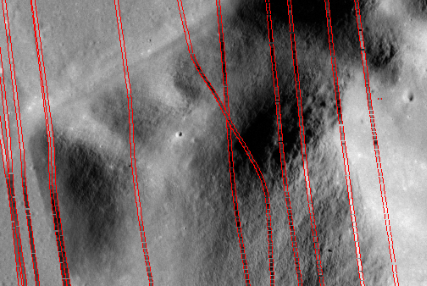
\includegraphics[width=0.5\columnwidth]{lidar2img/fig/mons_hadley_original_c.png}
	\label{fig:monshadleyoriginal}}
	\subfloat[After Coregistration]{
	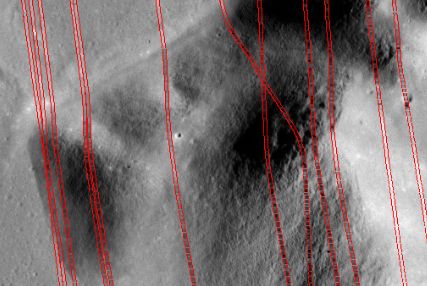
\includegraphics[width=0.5\columnwidth]{lidar2img/fig/mons_hadley_adjusted_c.png}
	\label{fig:monshadleyadjusted}}
	\caption{LOLA tracks passing through the western part of Mons Hadley are shown
		\subref{fig:monshadleyoriginal} before coregistration, and
		\subref{fig:monshadleyadjusted} after coregistration. Note how after
		coregistration, the synthetic image matches the actual image much more closely.}
	\label{fig:monshadley}
\end{figure}

\begin{figure}
	\centering
	\subfloat[Before Coregistration]{
	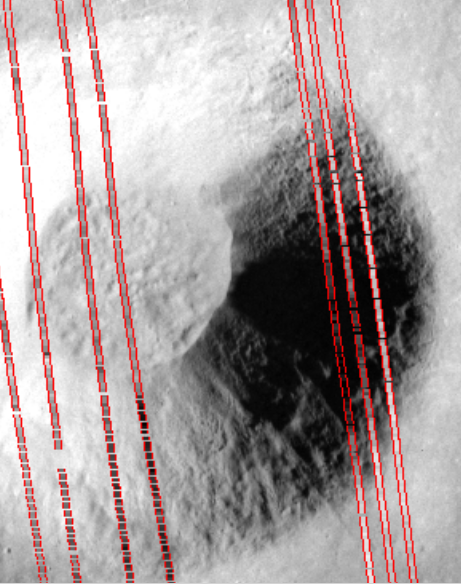
\includegraphics[width=0.5\columnwidth]{lidar2img/fig/aratus_original.png}
	\label{fig:aratusoriginal}}
	\subfloat[After Coregistration]{
	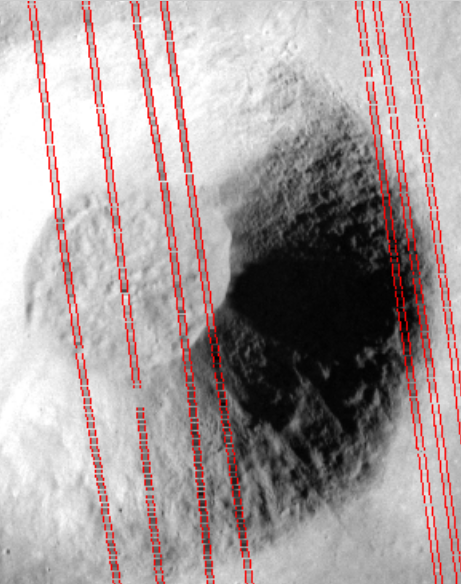
\includegraphics[width=0.5\columnwidth]{lidar2img/fig/aratus_adjusted.png}
	\label{fig:aratusadjusted}}
	\caption{LOLA tracks over Aratus crater
		\subref{fig:monshadleyoriginal} before coregistration, and
		\subref{fig:monshadleyadjusted} after coregistration. The sides of the
		crater form distinctive visual features.}
	\label{fig:aratus}
\end{figure}

% TODO: numeric error
Although our algorithm allows us to find general planar homographies from the track coordinates to
image coordinates, in practice the transformations that are found are affine transformations. They
have a large translational component and a slight rotational component.

